\documentclass[runningheads,a4paper]{llncs}

\usepackage{amssymb}
\setcounter{tocdepth}{3}
\usepackage{graphicx}

\usepackage{url}
\newcommand{\keywords}[1]{\par\addvspace\baselineskip
\noindent\keywordname\enspace\ignorespaces#1}

% Additional packages
\usepackage[utf8]{inputenc}
\usepackage{subfig}
\usepackage[pdftex,pdfpagelabels,bookmarks,hyperindex,hyperfigures]{hyperref}
\hypersetup{%
   plainpages=false, 
   pdfpagelayout=SinglePage,
   bookmarksopen=false,
   bookmarksnumbered=true,
   breaklinks=true,
   linktocpage,
   colorlinks=true,
   linkcolor=blue,
   urlcolor=blue,
   citecolor=blue,
   anchorcolor=green
}      

\begin{document}

\mainmatter  % start of an individual contribution

% first the title is needed
\title{Novelty Detection Using Graphical Models for Semantic Room Classification}

% a short form should be given in case it is too long for the running head
% \titlerunning{Lecture Notes in Computer Science: Authors' Instructions}

% the name(s) of the author(s) follow(s) next
%
% NB: Chinese authors should write their first names(s) in front of
% their surnames. This ensures that the names appear correctly in
% the running heads and the author index.
\author{Removed for Blind Review}
%\author{André Susano Pinto, Andrzej Pronobis, Luis Paulo Reis}
%
%\authorrunning{Lecture Notes in Computer Science: Authors' Instructions}
% (feature abused for this document to repeat the title also on left hand pages)

% the affiliations are given next; don't give your e-mail address
% unless you accept that it will be published
\institute{Removed for Blind Review}
%\institute{Faculdade de Engenharia da Universidade do Porto, Portugal\\
%\url{andresusanopinto@gmail.com}\\
%\url{http://url}}

\maketitle


\begin{abstract}
This paper presents an approach to the problem of novelty
detection in the context of semantic room categorization.
The ability to assign semantic labels to areas in the environment is crucial for
autonomous agents aiming to perform complex human-like tasks and human
interaction.
However, in order to be robust and naturally learn the semantics from
the human user, the agent must be able to identify gaps in its own knowledge.
To this end, we propose a method based on graphical models to identify novel
input which does not match any of the previously learnt semantic descriptions.
The method employs a novelty threshold defined in terms of conditional
and unconditional probabilities. The novelty threshold is then optimized using
an unconditional probability density model trained from unlabelled data.


\keywords{novelty detection, semantic data, probabilistic graphical models,
room classification, indoor environments, robotics, multi-modal classification.}
\end{abstract}


%%%%%%%%%%%%%%%%%%%%%%%%%%%%%%%%%%%%%%%%%%%%%%%%%%%%%%%%%%%%%%%%%%%%%%
\section{Introduction}

There has been several efforts in the areas of artificial intelligence and robotics
in creating robots that are able to interact with humans and their environments.
One of the important aspects is to endow those robots with a deeper understanding
of human environments, not just for the purpose of navigation and obstacle avoidance, 
but also in terms of human semantics and functionality. An important problem
in creating reliable representations of space for robots that are to be deployed 
in new and unknown realistic environments is to be able to automatically 
identify gaps in robot's knowledge and act in order to fill those gaps. 

This article addresses the problem of \emph{novelty detection} within the context
of semantic mapping i.e. generating maps containing \emph{semantic information} 
about indoor environments, such as homes or offices. In that context, the ability 
to detect that the observations result from a semantic concept unknown to the robot, 
and cannot be explained by one of its models, is crucial for generating fully autonomous
and reliable behavior. In order to be robust, the robot must identify 
novel concepts and instead of making a costly error, refrain from the decision
and initiate learning. In particular, we address the problem of novelty detection for
room categorization i.e. detecting whether the area in the environment identified as a
separate room can be assigned one of the semantic labels that the robot knows (e.g. as \emph{a kitchen} 
or \emph{an office}) or belongs to a yet unknown semantic category.


The novelty detection algorithm is implemented within a cognitive robot Dora the Explorer,
which already possesses a developed architecture based on probabilistic graphical models 
oriented towards dealing with uncertain semantic information and reasoning about it~\cite{ijcai}.
One of the major problems in using the probabilistic models of the environments for novelty
detection is selecting the optimal threshold above which the test sample is considered
novel. This problem becomes more difficult when, as in case of Dora, the representation
grows as the robot explores the environment. Methods are required to find
optimal parameters given the current structure of the model. To this end, this work 
studies methods for novelty threshold selection using probabilistic graphical models.

The rest of this paper is structured as follows. First, we briefly review the related work on
room categorization and novelty detection (Section~\ref{sec:related}). Then, we give an outline of the 
architecture of Dora and the structure of the conceptual map representing the semantic information
(Section~\ref{sec:overview}). Next, we discuss the methods for novelty detection (Section~\ref{sec:novelty-detection}) 
and present results of our preliminary experiments (Section~\ref{sec:results}). This paper concludes with a 
summary in Section \ref{sec:conclusion}.


%%%%%%%%%%%%%%%%%%%%%%%%%%%%%%%%%%%%%%%%%%%%%%%%%%%%%%%%%%%%%%%%%%%%%%
\section{Related Work}
\label{sec:related}
% TODO(pronobis): general comment about many .... approches to place categorization.
The problem of room categorization based on visual information was first addressed
in the computer vision community. In this case, the research focused mainly on the
problem of classifying single images captured in indoor or outdoor environments
(scene classification)~\cite{oliva2006building,torralba2003contextual}.
At the same time, robotics researchers initially employed
the 2D laser range sensor being much more robust to variations occurring in the
environment and much easier to handle computationally in real time~\cite{mozos2005supervised}.

Multi-modal approaches, such as combining semantic data extracted from
several sources or classifiers are expected to have better performance on scene
recognition than single-cue approaches. Quattoni and Torralba~\cite{quattoni2009recognizing}
showed that most scene recognition models work poorly in indoor scenes when
compared to outdoor scenes since the properties that
characterize rooms changes depending on the category. For instance corridors are well
described by global properties and bookstores are well described by the presence of
specific objects (books).
Galindo et al.~\cite{galindo2005multi} also exploits this by defining a bidirectional relation
between object and room category, where object defines a room category and a room
category provides information on where objects may be found.

Probabilistic representations have been frequently used for spatial modelling
in robots operating in the real-world~\cite{gross2009toomas,maier2010probabilistic}.
Boutell et al.~\cite{boutell2006factor} have studied outdoor scene classification using
\emph{factor graphs} and modelling spatial relations between objects in the scene
to extract better knowledge from semantic (high-level) features.

Although our approach is presented in the context of mobile robotics it relies on
standard concepts and techniques such as semantic data and graphical models.
Those are often used in the area of information retrieval.
An interesting example is the usage of an hidden concept layer between visual features
and text information to provide automatic image annotation~\cite{zhang2006probabilistic}.

Novelty detection has been studied for many years and there are several approaches
based on statistical analysis~\cite{markou2003novelty}.
Graphical models have been used to learn distributions of variables, both in
supervised and unsupervised ways and by using thresholds on those distributions
based solely on the conditional probability, as seen on Bishop~\cite{bishop1994novelty},
a novelty system can be trivially implemented.

However to the knowledge of the authors there is no reference on how to perform
novelty detection using graphs that are dynamically generated.
% TODO(andresp): anything more that can be said on why this paper is useful?

%%%%%%%%%%%%%%%%%%%%%%%%%%%%%%%%%%%%%%%%%%%%%%%%%%%%%%%%%%%%%%%%%%%%%%
\section{Dora Architecture Overview}
\label{sec:overview}

\begin{figure}[h]
\centering
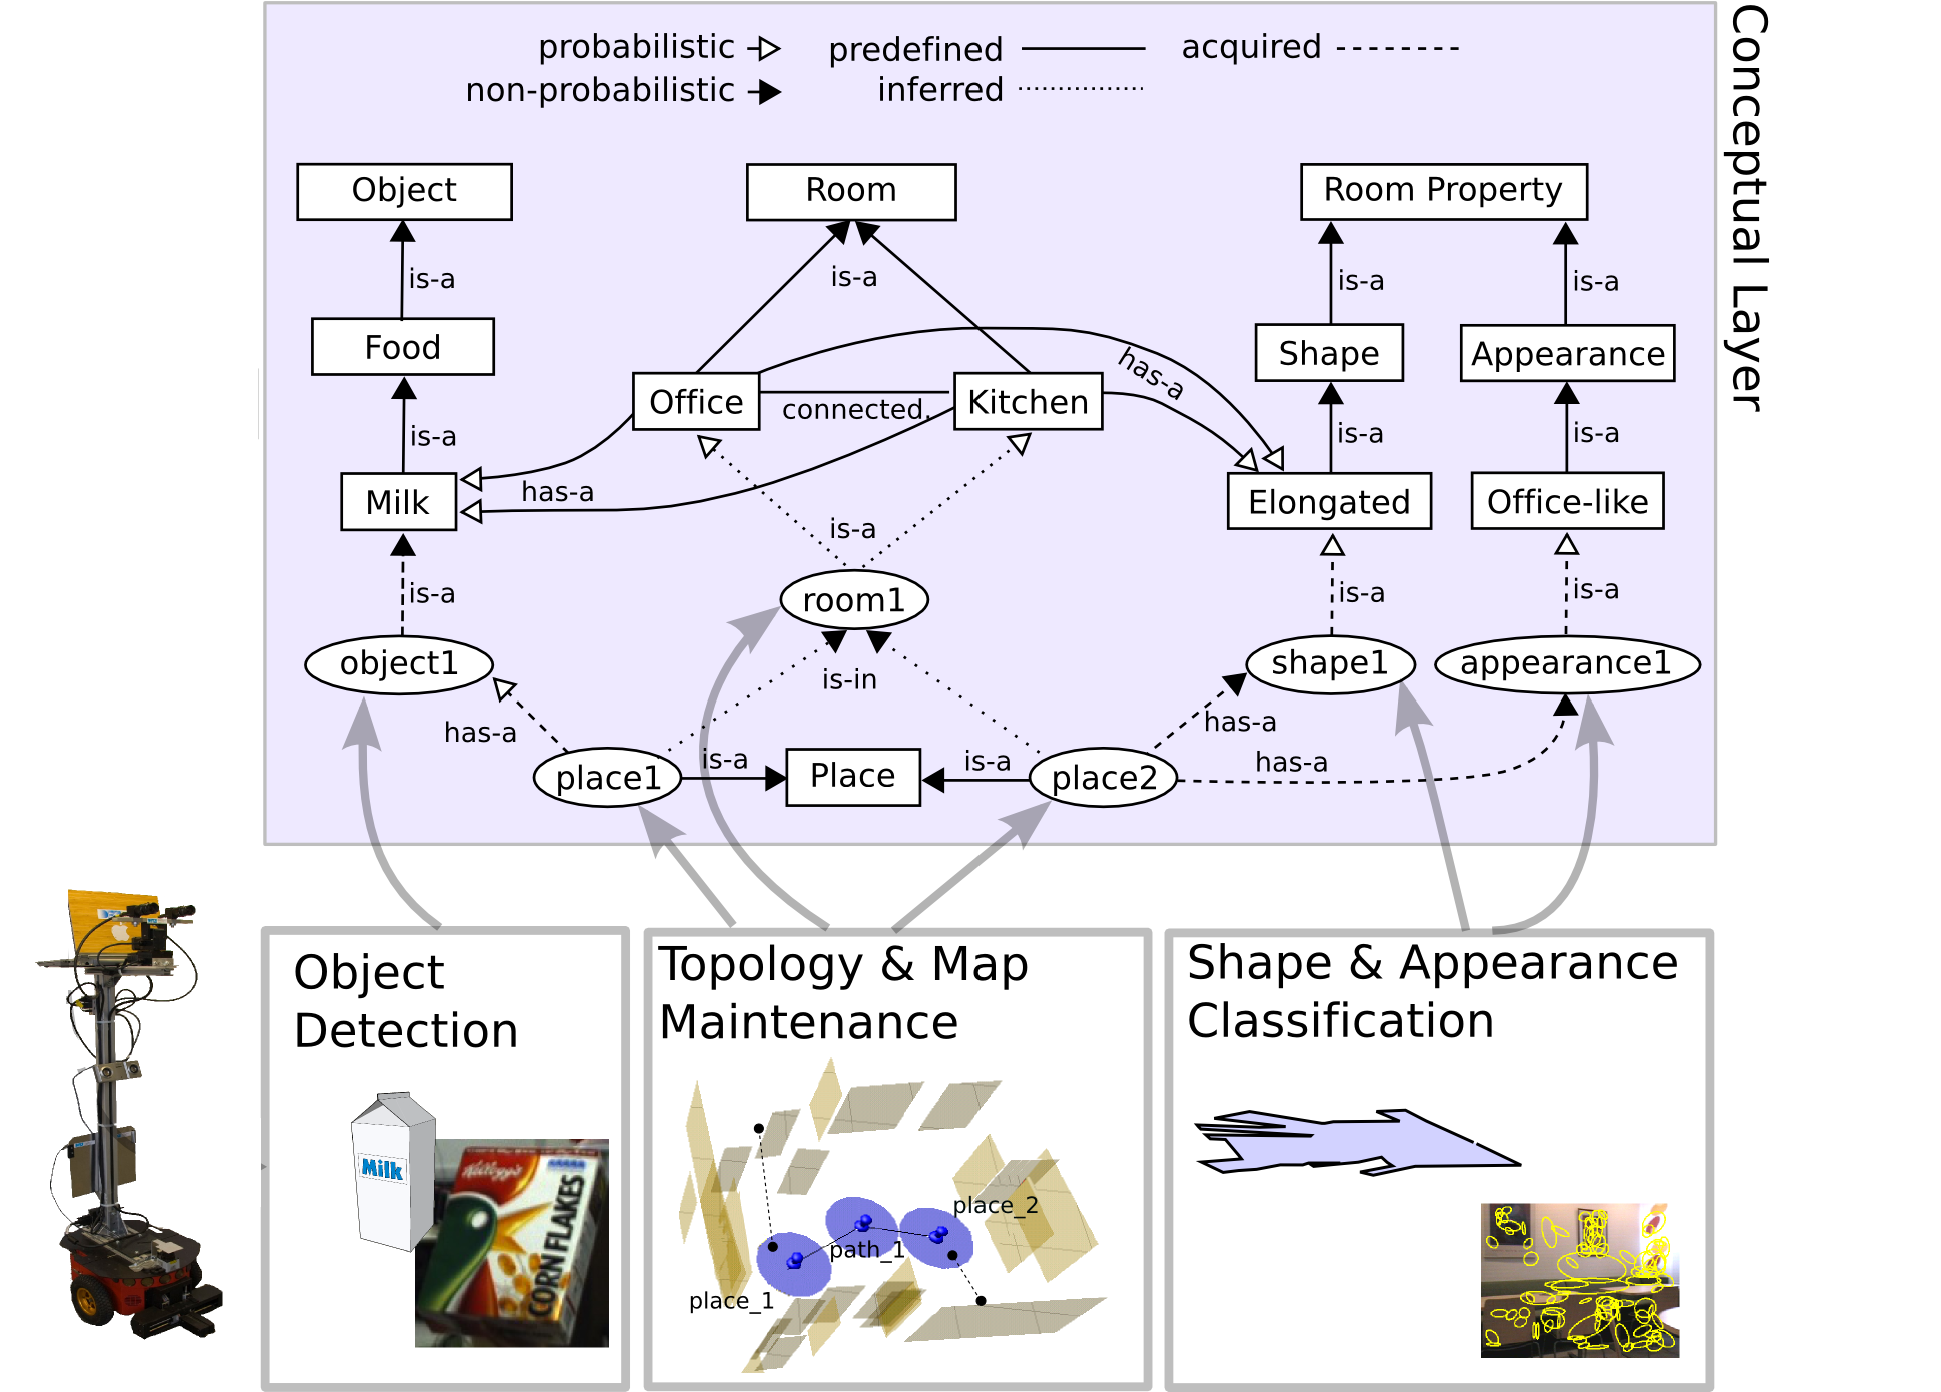
\includegraphics[width=0.9\textwidth]{figures/processes.pdf}
\caption{\label{fig:conceptual-layer}Interaction of the sub-systems
         in Dora with special focus on the conceptual layer.}
\end{figure}

The Dora system~\cite{ijcai} consists of several co-operating sub-systems,
all of which actively use or maintain the spatial knowledge representation
(see \autoref{fig:conceptual-layer}).
Only the \emph{conceptual layer} of the representation is of interest to this article.
Its role is to aggregate the following semantic information coming from other sub-systems:
\begin{description}
 \item[Doorway detection] is used to segment the continuous space into rooms and map connectivity between them.
 \item[Room size and shape] are classified by using 2D laser scans data from laser range finder mounted on the robot and are used as properties of a given room. The system utilizes pre-trained set of classifiers to extract rooms sizes (either large, medium or small) and shapes (rectangular or elongated).
 \item[Object detection] is performed in the images acquired by the robot through its camera. The system keeps track of the number of objects of each type in each room. Objects are detected by running a pre-trained set of detectors for the following object types: book, cereal box, computer, robot, stapler, toilet paper.
 \item[Room appearance] is categorized from the visual input by using global visual features and a pre-trained set of 7 different models.
\end{description}

As Dora moves through the environment its \emph{conceptual layer} builds a structural and
probabilistic representation of the space instantiated as a \emph{graphical model}.
It includes taxonomy of human-compatible spatial concepts which are linked to the sensed 
instances of these concepts drawn from lower layers. It is the conceptual layer which 
contains the information that kitchens commonly contain cereal boxes and have certain 
general appearance and allows the robot to infer that the cornflakes box in front of the 
robot makes it more likely that the current room is a kitchen. The conceptual layer is 
described in terms of a probabilistic ontology defining spatial concepts and linking 
those concepts to instances of spatial entities (see the example of the ontology in
\autoref{fig:conceptual-layer}).

\subsection{Conceptual Map}

Based on this design, a \emph{chain graph}~\cite{lauritzen2002chain} model is proposed as a 
representation for performing inferences on the knowledge represented in the conceptual 
layer. Chain graphs are probabilistic graphical models that combine the properties of 
both Bayesian Networks and Random Markov Fields. This results in an efficient approach to 
probabilistic modeling and reasoning about conceptual knowledge.

\begin{figure}[h]
\centering
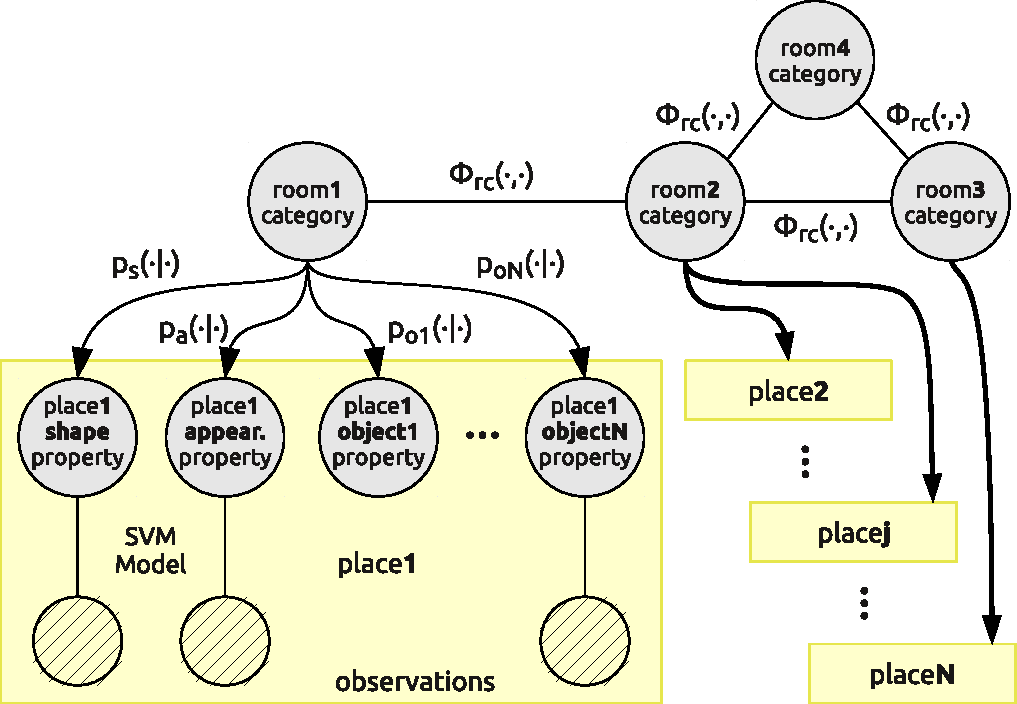
\includegraphics[width=0.80\textwidth]{figures/chaingraph.pdf}
\caption{\label{fig:chain-graph}Example chain-graph produced by the \emph{conceptual layer}.}
\end{figure}

%The conceptual layer structures the sensed environment together with the conceptual knowledge
%in order to create a structured probabilistic representation of the world.
An exemplary chain graph corresponding to the conceptual map ontology is presented
in \autoref{fig:chain-graph}. 
Each discrete place identified in the environment is represented by a set of random variables, 
one for each class of relation linked to that place. These are each connected to a random variable
over the categories of rooms, representing the ``is-a'' relation between rooms and their categories. 
Moreover, the room category variables are connected by undirected links to one another according 
to the topological map. The remaining variables represent: shape and appearance properties of space 
as observed from each place, and the presence of objects. 
These are connected to observations of features extracted directly from 
the sensory input. Finally, the 
distributions $p_{s}(\cdot|\cdot)$, $p_a(\cdot|\cdot)$, $p_{o_i}(\cdot|\cdot)$ 
represent the common sense knowledge about shape, appearance, and object co-occurrence, respectively. 
They allow for inference about other properties and room categories e.g. that the room is likely to be a kitchen,
because you are likely to have observed cornflakes in it. 

The use of graphical models to describe distributions of variables has useful properties.
First, they permit inference about uncertain conceptual knowledge. At the same time, they are 
generative models and therefore allow to calculate the probability
on any given subset of variables of the graph, allowing the system to work even when some
information is missing.


\subsection{Factor Graphs}
Although the conceptual layer works with \emph{chain graphs}, those can be converted
into \emph{factor graphs}~\cite{kschischang2001factor}. Factor graphs are used throughout this paper as they provide an
easier manipulation due to factorization.
Moreover, there exists efficient implementation of inference engines operating on factor graph
representations~\cite{Mooij_libDAI_10}.
Describing the distribution function in terms of graphs allows to use those engines to
efficiently calculate marginals on any given subset of variables by exploiting conditional
independence between variables.

A \emph{factor graph} is a bipartite graph connecting two sets of nodes $X_G$ and $F_G$
representing random variables and factors.
Each factor is described by function $\phi$ dependent only on the variables $x_\phi$
to which the factor is connected.
Thus, a factor graph can be seen as a description of probability density function obtained
by a product of all the factors. In order to represent the probability,
a normalization factor needs to be introduced, resulting in the following equation:

\begin{equation}
P_G(x) = \frac{1}{Z}\prod_{\phi \in F_G}{\phi(x_{\phi})},\qquad
Z = \sum_{X_G}\prod_{\phi \in F_G}{\phi(x_{\phi})}
\end{equation}


%%%%%%%%%%%%%%%%%%%%%%%%%%%%%%%%%%%%%%%%%%%%%%%%%%%%%%%%%%%%%%%%%%%%%%
\section{Novelty Detection}
\label{sec:novelty-detection}
% Introduce novelty detection
Novelty detection deals with detecting that a data sample belongs to a class
originated by a distribution other than the ones the system knows about~\cite{markou2003novelty}.
It is harder than classification as only positive samples of the class are available
rendering normal classification methods unusable.

Adding capabilities to an agent to detect novel samples allows to increase its
reliability. Novelty signal can then be interpreted by the system to proceed
with more caution as its knowledge does not correctly describe reality.

% Explain threshold approach to novelty detection
Due to the nature of the sensed data which are noisy and uncertain, novelty ought to be
treated in a probabilistic way where each sample has certain probability
of being generated by a class not known to the agent and a complementary probability $P(\overline{novel}|x)$
of being generated by a known class.
The true positive and false positive rate of a novelty detection system which classifies
the set $N$ of samples as novel is given by:

\begin{eqnarray}
P(\textnormal{true positive})  &=& \sum_{x \in N}{P(novel|x)P(x)} \\
P(\textnormal{false positive}) &=& \sum_{x \in N}{P(\overline{novel}|x)P(x})
\end{eqnarray}

It leads that by extending the set $N$ with new samples, the true positive and
false positive rate can never be decreased, leading to the problem where in order
to increase detection a system needs to increase its error. This describes the
base of the \emph{error and rejection tradeoff}~\cite{chow1970optimum}, which
states that a system aiming at increasing the true-positive probability will eventually increase its
false-positive error.

This way an optimal detector can be formulated by achieving the maximum true-positive
probability without its false-positive probability increasing beyond a given limit.
This is equivalent to a \emph{continuous knapsack problem} which allows a greedy
solution by sorting the items with a value per weight function. In the case of 
detection system that can be defined as:

\begin{eqnarray}
value(x)  &=& P(novel|x) \\
weight(x) &=& P(\overline{novel}|x) \\
cost(x)   &=& value(x)/weight(x) \\
          &=& \frac{P(novel|x)P(x)}{P(\overline{novel}|x)P(x)}
\end{eqnarray}

Therefore a novelty detection system before classifying a sample $a$ as novel should (greedily)
classify any sample $b$ with a smaller cost as that would achieve a higher true positive probability 
given a fixed false positive one.

\begin{equation}
\label{eq:knapsack}
\frac{P(novel|b)}{P(\overline{novel}|b)} < \frac{P(novel|a)}{P(\overline{novel}|a)}
\end{equation}

This relation between $a$ and $b$ can further be simplified into:

\begin{equation}
P(\overline{novel}|b) < P(\overline{novel}|a)
\end{equation}


Based on this, it can be said that an optimal novelty detection system is
interested in defining an order relation on all the possible inputs equivalent
to the order defined by the function: $P(\overline{novel}|x)$.
And any optimal detector can be described by the largest $P(\overline{novel}|x)$
accepted by it. This can be seen as thresholding.

Using Bayes rule and assuming a constant $P(\overline{novel})$
a ratio between a conditional and unconditional probabilities of the input $x$ is obtained.
Such a ratio is a suitable function for implementing a novelty detector system with optimal
thresholding.

\begin{equation}
\label{eq:novelty-threshold}
          P(\overline{novel}|x)
  =       \frac{P(x|\overline{novel}) P(\overline{novel})}{P(x)}
  \propto \frac{P(x|\overline{novel})}{P(x)}
\end{equation}

Note, however that in the case of dynamic graph structures, an assumption on a constant
$P(novel)$ is quite strong. And although on this first approach it is assumed to be
constant, the authors acknowledge that structure plays an important role and should
be used as prior-information when calculating $P(novel)$.

% Explain approach of using conditional probability
\subsection{Conditional Probability}
\label{sec:conditional-prob}
The conditional probability models the distribution of variables given that the sample
is not novel for the agent.
This is: it should model the distribution of the sensed features considering that the
knowledge the agent possesses holds true. Under that its natural to model it with a graphical
model that combines the information acquired with the relations that the describe the
relations learned by the agent between the variables.

In Dora case, this is equivalent to use the graphical model used by it to describe its
current believes on the variables modelled by the system.
That graph is built, by the conceptual layer, by instancing the information extracted from
other layers together with the conceptual knowledge such as: objects are properties of rooms,
rooms are connected between each other.

\begin{figure}[h]
\centering
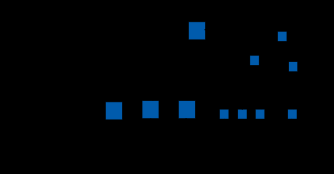
\includegraphics[width=0.65\textwidth]{figures/conditional-prob-graph.pdf}
\caption{\label{fig:conditional-prob-graph}Illustration of a factor graph modelling
         a distribution of a set $x$ of sensed variables.}
\end{figure}

\autoref{fig:conditional-prob-graph} illustrates a graph $G$ built from the conceptual
layer to represent the conditional probability on the sensed variables $x$.
A set of hidden variables is added to represent the conceptual knowledge the system is aware of.
In the presented graph variables $R_i$ were added to model the room categories that influence
the directly sensed features on each physical room, as well connectivity factors between each
room.

The factors connecting the variables are trained by the system by searching databases of
common knowledge to build potentials describing how likely it is that a specific set of
values for a set of variables is likely to occur.
For instance: it is very likely to find a cereal box in a kitchen; and it is unlikely to find
bathroom connected to another bathroom.
We propose using such a graph $G$ built by the conceptual layer for modelling $P_G(x)$
as an approximation for $P(x|\overline{novel})$.

\subsection{Unconditional Probability}
\label{sec:unconditional-prob}
With only access to labelled data a common approach is to define a threshold assuming
that $P(x)$ is constant through all the samples.

Its important to notice that in several cases assuming it to be constant leads to
discarding the factor.
Nonetheless, here the distributions are dynamically changing as the system learns
more on the environment.
So the normalizing argument $P(x)$ has to be evaluated for each new subset of $x$.

Assuming that the unconditional distributions generates all possible outcome with
the same probability we can model it with $\prod{1/\# x_i}$,
where $\# x_i$ denotes the cardinality of the state space of variable $x_i$.
In graphical model terms this is represented to a factor graph $U$ with the
variables but without any factors as illustrated on \autoref{fig:uniform-prob-graph}.

\begin{figure}[h]
\centering
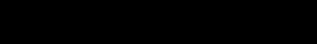
\includegraphics[width=0.65\textwidth]{figures/uniform-prob-graph.pdf}
\caption{\label{fig:uniform-prob-graph}Without any existing factors, this graph $U$ represents a
         uniform distribution over any set of its variables.}
\end{figure}

Having a graphical model $G$ built to model the known data distribution and a model
$U$ for the unconditional probability a novelty threshold would be given by:
$P_G(x)/P_U(x)$.
Here $P_{U}(x)$ can be seen as a normalizing factor to lever all the $P_G(x)$ on any set of
variables $x$ into the same measure units (error rate), such that a static threshold can be implemented.
For example the conditional probability would yield very small values on large sets of variables
$x$ than in small sets due to the spreading over the dimensions of the sample space.
As so a novelty measure is seen as a ratio on how much introducing the known concepts helps to
understand the observed result.


\subsection{Semi Supervised: Using Unlabelled Data}
Nonetheless, its often the case that there is access to extra data that allows to
obtain a better approximation to the unconditional probability than the uniform one.
In specific, all the knowledge of the agent can be considered to hold true apart from
complete knowledge on the categories of a room.
In that case a single big factor can be used to model all the variables directly
dependent on the room which the category cannot be assumed to be known as illustrated in
\autoref{fig:unconditional-prob-graph}.

\begin{figure}
\centering
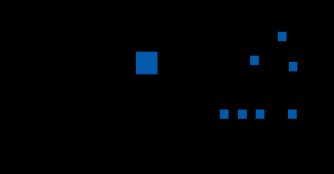
\includegraphics[width=0.65\textwidth]{figures/unconditional-prob-graph.pdf}
\caption{\label{fig:unconditional-prob-graph}Without being able to model variable $R_1$
all the variables directly dependent on it become dependent between each other introducing
a single big factor.}
\end{figure}

For practical reasons it is impossible to train such a factor, and simplifications need
to be performed. And here, it was assumed that it can be approximated by factorizing
it in several single factors such that all variables become independent.
Additionally those single factors can easily be trained by using unlabelled data,
obtaining this way a graphical model $I$,
as illustrated in \autoref{fig:single-unconditional-prob-graph},
to be used as approximation for the unconditional probability.

\begin{figure}[h]
\centering
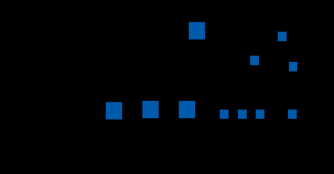
\includegraphics[width=0.65\textwidth]{figures/single-unconditional-prob-graph.pdf}
\caption{\label{fig:single-unconditional-prob-graph}By factorizing the single factor
introduced by room 1 not being necessarily known, several single factors are obtained
that can be trained from unlabelled data.}
\end{figure}

Once again the novelty threshold would be given by $P_G(x)/P_I(x)$.
This time the addition of the unconditional factors can be understood as an
attempt to compensate for an existing bias on the unconditional distribution.
This is an important step to achieve a correct order-relation of the inputs sample
for implementing a novelty threshold.


%%%%%%%%%%%%%%%%%%%%%%%%%%%%%%%%%%%%%%%%%%%%%%%%%%%%%%%%%%%%%%%%%%%%%%
\section{Results}
\label{sec:results}

In order to verify the performance of the proposed threshold functions a synthetic dataset
was generated. As the point on this initial work was only to test the correctness of
the presented threshold function and approximation capabilities by using a uniform or
an independent model, only information regarding direct features of a room were
modelled and no structured knowledge such as room connectivity was taken
in account.

The synthetic distribution assumes that an independent and variable number of features
$x$ is generated by a given room category.
In whole there was 11 different room categories and 9 different measured feature
types. The number of sensed features is dynamic and mimic the type of information
extracted when running on the robot. Due to that it is possible that on a given sample
a certain feature type can be present more than once or not be present at all
(e.g.: room shape is extracted from 2D laser scans in more than one position in the room,
information about detected objects is only present when the robot previously tried to
detect objects on a given room).

The sensed properties and room categories were chosen to mimic as close as possible
the reality and they are based on a previously build ontology from web data.
There is in total 11 different room categories ranging from: corridor, hallway,
1 person office, 2 person office, bathroom, conference hall, etc\dots, and there is
9 different extracted features: room size, room shape, room appearance and 6 different objects
(e.g. book, cereal box, computer).

From the distribution, 100 labelled samples for 5 of the 11 room categories were
drawn to represent the known categories and 1000 unlabelled samples were drawn from
all the room categories for learning the unconditional probability distribution.
Using those samples, factors were learnt for the graphs used to model the
conditional distribution and the independent unconditional distribution.
\autoref{fig:simple-experiment} shows the graph structure used for approximate the
trained conditional and unconditional distributions.
Its important to notice that graph $G$ used to model the known classes when given
enough labelled data is able to exactly learn the conditional distribution as it
uses the same structure as the created synthetic distribution.

\begin{figure}[h]
\centering

\subfloat[Graph structure $G$.]{
         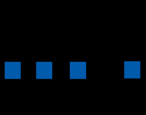
\includegraphics[width=0.27\textwidth]{figures/simple-cond-graph.pdf}}
\qquad
\subfloat[Graph structure $U$.]{
         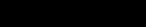
\includegraphics[width=0.27\textwidth]{figures/simple-uniform-graph.pdf}}
\qquad
\subfloat[Graph structure $I$.]{
         
\includegraphics[width=0.27\textwidth]{figures/simple-independent-graph.pdf}}

\caption{\label{fig:simple-experiment}The graph structures used to model the
         conditional and unconditional probability for implementing the novelty
         thresholds $P_G(x)/P_U(x)$ and $P_G(x)/P_I(x)$.}
\end{figure}

% Describe how to obtain the 3 thresholds functions seen on the graphs.
Using the learned models $G$, $U$ and $I$, two thresholds were trained:
$P_G(x)/P_U(x)$ assuming a uniform unconditional distribution
and $P_G(x)/P_I(x)$ assuming an independent unconditional distribution.
Since the distribution is synthetic there is access to $P(x)$ and $P(x|\overline{novel})$
and a perfect threshold function could also be created to test how far the
presented thresholds are from optimal.

\subsection{Probability Ratio Comparison}
%%% Results 1
% Show the threshold ratio is an optimal detector (if perfect information was available)
% Show that the thresholds are suitable functions for implementing a static threshold.
First, the performance of the novelty threshold selection was plotted for a set
of 1000 samples taken from the whole distribution (\autoref{fig:synthetic-roc}).
The samples where uniformly generated by graphs with 5, 10, 15, 20, 35, 50 features.
Additionally the feature types were also uniformly sampled, for that it is possible
that in certain samples some feature types were sensed more than once and other were not
sensed at all.
This was chosen to mimic
the dynamic properties expected to see when implemented on a robot.

\begin{figure}[h]
\centering
\includegraphics[width=0.60\textwidth]{results/synthetic-all.pdf}

\caption{\label{fig:synthetic-roc}ROC curve comparing novelty detection performance
         under samples with variable size of sensed properties.}
\end{figure}


The convex shape of the optimal threshold shows that the ratio between conditional
and unconditional probability is indeed a suitable detector for implementing a threshold when
the samples are taken from dynamic distributions when $P(novel)$ is constant
(e.g.\ some samples where there is only access to room size versus
samples where there is a lot of information about the room properties).

% Discuss importance on approximating unconditional probability.
Its also possible to see how important it is to estimate a correct unconditional
probability in order to obtain a correct novelty measure on the inputs.
The assumption of a uniform unconditional probability has led to very poor results.
That is probably explained by the semantic properties being highly
biased towards some values. This shows that bias plays an important role
in detecting whether a given sensed value is a valuable cue about the room category.



%%% Results 2
% Measure performance of the thresholds as more information becomes available.
\subsection{Performance Changes With Amount of Available Information}
In order to measure the performance impact as more semantic information becomes
available, ROC curves were plotted for samples grouped by the number of sensed
semantic features.

\begin{figure}[h]
\centering

\subfloat[3 sensed features]{\includegraphics[width=0.40\textwidth]{results/synthetic-3features.pdf}}
\qquad
\subfloat[5 sensed features]{\includegraphics[width=0.40\textwidth]{results/synthetic-5features.pdf}}

\subfloat[10 sensed features]{\includegraphics[width=0.40\textwidth]{results/synthetic-10features.pdf}}
\qquad
\subfloat[50 sensed features]{\includegraphics[width=0.40\textwidth]{results/synthetic-50features.pdf}}

\caption{\label{fig:synthetic-roc-breakdown}ROC curves plotted showing performance of the
         presented novelty detection method for graphs generated for different amount of
         sensed features.}
\end{figure}

It is possible to see that as the system gains more semantic information, it
becomes easier to detect novelty. The size of the input space increases and allows the
existing classes to become more easily distinguished.

The performance of the independent threshold decreases as the number of sensed
features increases. This is easily explained by the fact that the graph $I$ is not
able to model the existent dependence between the features. This becomes obvious
as the number of features increases (e.g.\ graph $I$ perfectly models $P(x)$ in the
case where only 1 feature is sensed).

The uniform threshold shows poor performance especially for samples with small amount of features
where it performs almost no better than random.
The performance increases as the size of sensed features increases but nonetheless
is very small when compared to the optimal threshold.


%%%%%%%%%%%%%%%%%%%%%%%%%%%%%%%%%%%%%%%%%%%%%%%%%%%%%%%%%%%%%%%%%%%%%%
\section{Conclusions and Future Work}
\label{sec:conclusion}
In this paper we presented how to define a stable novelty threshold function on
top of \emph{probabilistic graphical models} instantiated dynamically from sensed
semantic data.
The presented technique is based on the ratio between a conditional and
unconditional probability and when perfect information exists it performs an optimal
novelty detection threshold.

It was also shown that a correct estimation of unconditional probability plays an
important role specially on small input spaces. Moreover, semi-supervised techniques
implemented with the access to unlabelled data can be used to significantly improve
novelty detection performance.

Given the synthetic distribution, an assumption on an uniform
distribution has led to very poor results. The same behaviour is expected to
in real world distributions based on semantic data. For that reason,
and due to easy access to unlabelled data, special attention will be given to using
semi-supervised techniques for novelty detection.

After this initial study on how to detect new semantic classes based on
graphical models, future work will focus on how to use the structured
information available from the conceptual layer to be able to detect which variable
of the graph is novel and what makes it different from other previously learned
classes. That will lead to generation of useful information that can be used for
communication with the user and performing active learning of new room categories.


%%%%%%%%%%%%%%%%%%%%%%%%%%%%%%%%%%%%%%%%%%%%%%%%%%%%%%%%%%%%%%%%%%%%%%
\bibliographystyle{unsrt}
\bibliography{refs}

\end{document}
